\documentclass[12pt]{article}
\usepackage{amsmath}
\usepackage{graphicx}
\usepackage{amsfonts}
\usepackage{hyperref}
\usepackage{geometry}
\usepackage{listings} 
\usepackage{placeins}
\usepackage[T1]{fontenc}

\geometry{top=2.5cm, bottom=2.5cm, left=2.5cm, right=2.5cm}

\title{Signal Synthesis Using Inverse Discrete Fourier Transform (IDFT)}
\author{Daria Kręcichwost}
\date{\today}

\begin{document}

\begin{titlepage}
    \centering
    \vspace*{2cm}
    
    \Huge
    REPORT
    
    \vspace{1cm}
    
    \Large
    Course: Analog and digital electronic circuits \\
    Teacher: Prof. Dr. Hab. Vasyl Martsenyuk
    
    \vfill
    
    \Large
    Lab No. 1 and 2\\
    Date: \today \\
    Topic: "Figures Demonstrating Fourier Transform" \\
    Variant: 8
    
    \vspace{1cm}
    
    \large
    Name: Daria Kręcichwost \\
    Computer Science (Second Degree) \\
    Part-time studies, Semester 1 \\
    Group: B
\end{titlepage}

\newpage

\maketitle


\section{Problem Statement}
The task involves synthesizing discrete-time signals from their DFT coefficients using the Inverse Discrete Fourier Transform (IDFT) in matrix notation. The goal is to reconstruct time-domain signals from frequency-domain sequences \( \mathbf{X}_\mu \) and visualize the results, including real and imaginary parts.

\section{Input Data}
The input data for this task is a sequence of DFT coefficients \( \mathbf{X}_\mu \), defined as follows:
\[
\mathbf{X}_\mu = [6, 2, 4, 4, 4, 5, 0, 0, 0, 0]
\]
The corresponding time-domain signal is computed using the IDFT. The task also involves plotting the synthesized signal for analysis.

\section{Commands used (or GUI)}
The following Python code was used to synthesize signals from the input DFT coefficients using the IDFT:

\begin{lstlisting}[language=Python, breaklines=true]
import numpy as np
import matplotlib.pyplot as plt

def idft_matrix(N):
    W_N = np.exp(-2j * np.pi * np.outer(np.arange(N), np.arange(N)) / N)
    return W_N

def synthesize_signal(X_mu):
    N = len(X_mu)
    W_N = idft_matrix(N)
    x_mu = np.dot(W_N.conj().T, X_mu) / N
    return x_mu

X_mu = np.array([6, 2, 4, 4, 4, 5, 0, 0, 0, 0], dtype=complex)

x_mu_synthesized = synthesize_signal(X_mu)

plt.figure(figsize=(10, 6))
plt.stem(np.real(x_mu_synthesized), linefmt='b-', markerfmt='bo', basefmt='r-')
plt.title('Synthesized Signal (Real Part)')
plt.xlabel('Sample Index')
plt.ylabel('Amplitude')
plt.grid(True)
plt.show()

plt.figure(figsize=(10, 6))
plt.stem(np.imag(x_mu_synthesized), linefmt='g-', markerfmt='go', basefmt='r-')
plt.title('Synthesized Signal (Imaginary Part)')
plt.xlabel('Sample Index')
plt.ylabel('Amplitude')
plt.grid(True)
plt.show()

plt.figure(figsize=(12, 6))
plt.plot(np.real(x_mu_synthesized), label='Real Part', marker='o', linestyle='-', color='b')
plt.plot(np.imag(x_mu_synthesized), label='Imaginary Part', marker='x', linestyle='--', color='g')
plt.title('Signal Synthesis: Real and Imaginary Parts Combined')
plt.xlabel('Sample Index')
plt.ylabel('Amplitude')
plt.axhline(0, color='red', linewidth=0.8, linestyle='--', label='Zero Line')
plt.legend()
plt.grid(True)
plt.show()

\end{lstlisting}
\item \href{https://github.com/DariaKrecichwostQA/StudiaUBB/tree/main/Digital%20Signal%20Processing/Zad1}{{Link to remote repository on GitHub})}

\newpage
\section{Outcomes}
The synthesized signals were analyzed and visualized. The results include the real part, the imaginary part, and the combined representation of both.

\subsection{Real Part of the Signal}

\begin{figure}[htbp]
    \centering
    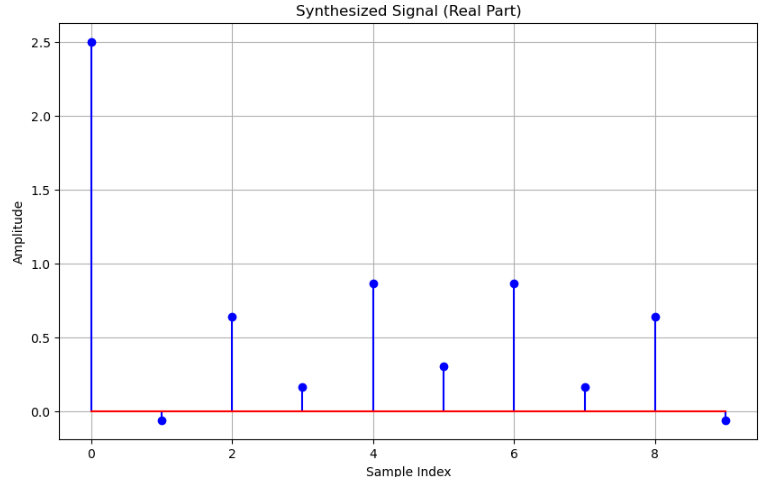
\includegraphics[width=0.8\textwidth]{1.png}
    \caption{Synthesized Signal (Real Part)}
    \label{fig:real_part}

\end{figure}
\newpage
\vfill
\subsection{Imaginary Part of the Signal}
\begin{figure}[htbp]
    \centering
    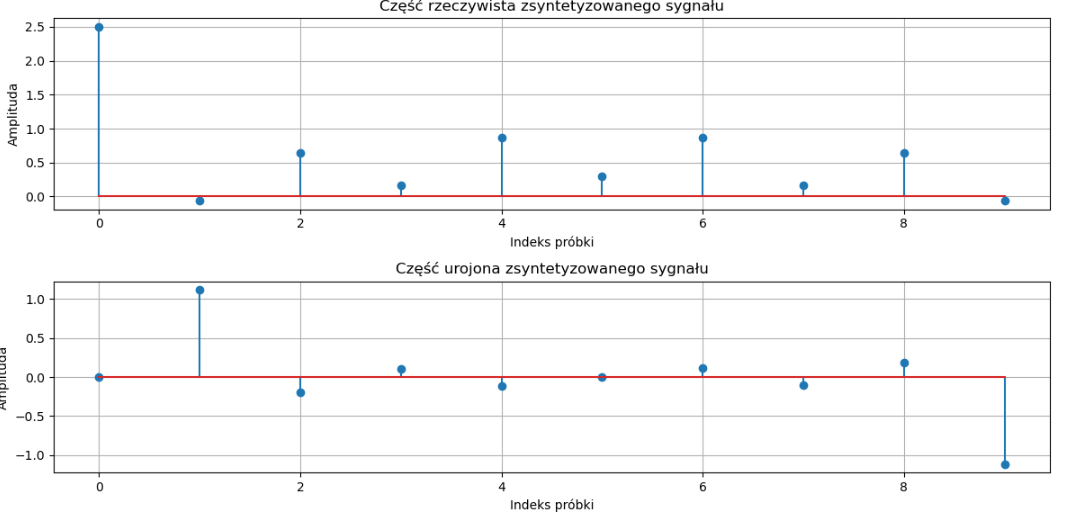
\includegraphics[width=0.8\textwidth]{2.png}
    \caption{Synthesized Signal (Imaginary Part)}
    \label{fig:imaginary_part}
\end{figure}

\FloatBarrier
\vfill
\newpage
\subsection{Combined Signal (Real and Imaginary)}
\begin{figure}[htbp]
    \centering
    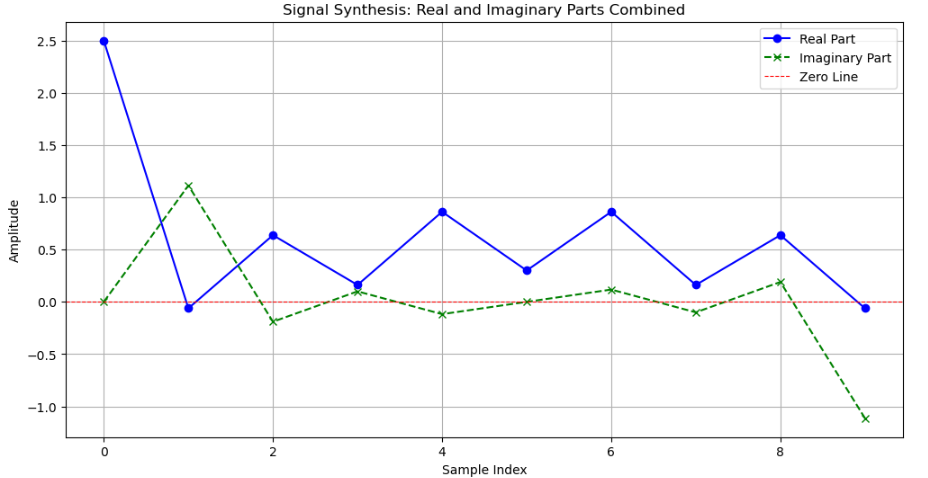
\includegraphics[width=0.8\textwidth]{3.png}
    \caption{Signal Synthesis: Real and Imaginary Parts Combined}
    \label{fig:combined_signal}
\end{figure}

\FloatBarrier
\vfill


\newpage

\section{Conclusions}

\begin{itemize}
    \item The comparison between the real and imaginary parts of the signal shows how these two components are interconnected in the signal synthesis process.
    \item The real part of the signal is more intuitive and easier to understand, as it reflects the signal's amplitude, while the imaginary part provides information about its phase.
    \item Both parts are essential to obtain a complete and accurate time-domain reconstruction of the signal.
    \item The zero line plays a crucial role in visualizing the signal's behavior, providing a reference point for identifying the positive and negative oscillations.
    \item The real and imaginary components fluctuate around this line, and it helps to better interpret the amplitude and phase changes, ensuring a more accurate understanding of the signal's characteristics.
\end{itemize}



\end{document}
